% !TeX TXS-program:compile = txs:///pdflatex/[--shell-escape]
\documentclass[12pt, a4paper]{article}

% IMPORTANT
% Set status of the doc
\def\draft{draft}
\def\final{final}
\def\status{draft}

% Include setup stuff
% !TeX root = ../main.tex
\usepackage{a4wide}

\usepackage[utf8]{inputenc}

%\usepackage[ngerman]{babel}
\usepackage[english]{babel}

\usepackage[T1]{fontenc}
\usepackage{palatino}

\usepackage{graphicx}
\usepackage{caption}
\usepackage{url}
\usepackage{tocloft}
\usepackage{acronym}

\usepackage{mathpazo}
\usepackage{amsmath}
\usepackage{amsfonts}
\usepackage{adjustbox}

%\usepackage{subcaption}

\usepackage{hhline}
\usepackage{amssymb}
\usepackage{floatflt}
\usepackage{setspace}
\usepackage{float}
\usepackage{color}
\usepackage{listings}
\usepackage{array}
\usepackage{scrhack}
\usepackage{xcolor}
\usepackage{wrapfig}
\usepackage{hyperref}
\usepackage{url}
\usepackage{lmodern}
\usepackage{multirow}
\usepackage{subfig}
\usepackage{cleveref}
\usepackage{lipsum}


% !TeX root = ../main.tex
%%%%%%%%%%%%%%%%%%%%%%%%%%%%%%%%%%%%%%%%%%%%%%%%%%%%%%%%%%%%%%%%%%%%%%%%
% Data about you and the Document%
%%%%%%%%%%%%%%%%%%%%%%%%%%%%%%%%%%%%%%%%%%%%%%%%%%%%%%%%%%%%%%%%%%%%%%%%

% % Main Title of Document:
\newcommand{\myMaintitle}{Untersuchung und Aufbau einer DevOps Development Umgebung}

% % Sub Title of DocInput:
\newcommand{\mySubtitle}{Developing holistic software solutions through integration of existing individual solutions.}

% % Ihr Name:
\newcommand{\myName}{Henrik Gerdes}

% % Matrikelnummer:
\newcommand{\myMatrikel}{MatNr: 969272}

% % Ihr Geburtsort:
\newcommand{\brith}{Osnabrück}

% % Ihr Geburtsort:
\newcommand{\place}{Osnabrück}

% % Ihr Abgabedatum:
\newcommand{\submission}{\today}

% % Ihr Abgabedatum:
\newcommand{\mycourse}{Exposé für den B.Sc.}

% % Name des Betreuers/Erstprüfenden:
\newcommand{\fistSupervisor}{Dennis Ziegenhagen}
\newcommand{\secSupervisor}{Achim Hendrix}

% % In welchem Semester befinden Sie sich?
\newcommand{\mySemester}{6. Semester}

\title{\myMaintitle}

\author{\myName}
% !TeX root = ../main.tex
% % Zeilenabstand im Haupttext auf anderthalb-zeilig setzen
%\linespread{1.25}\selectfont

% Line spacing
%\onehalfspacing{}

%Pfad für Grafiken
\graphicspath{{fig/}}

%Styleregeln
\widowpenalty10000 % Vermeidet einzelne Zeilen eines Absatzes zu Beginn einer Seite
\clubpenalty10000 % Vermeidet einzelne Zeilen eines Absatzes am Ende einer Seite
\addtocontents{toc}{\protect\sloppy}
\setcounter{tocdepth}{3}


% % \sloppy bewirkt, dass Latex beim Blocksatz nicht über den rechten Rand hinausschreibt.
% % und dafür größere Lücken in einer Zeile in Kauf nimmt
\sloppy

% % Setzt Dokumenteigenschaften für PDFs, wenn das Paket 'hyperref' geladen wurde.
\hypersetup{pdftitle=\myMaintitle,pdfauthor=\myName,bookmarksopen=true}

%Source for picture captions
\newcommand{\source}[1]{\caption*{Source: {#1}} }

\newcommand{\code}[1]{\texttt{#1}}

\newcommand{\myparagraph}[1]{\paragraph{#1}\mbox{}\\}

\newcommand{\RM}[1]{\MakeUppercase{\romannumeral{} #1{}}}

\newcommand{\HRule}{\rule{\linewidth}{0.5mm}} % Defines a new command for horizontal


\definecolor{dkgreen}{rgb}{0,0.6,0}
\definecolor{gray}{rgb}{0.5,0.5,0.5}
\definecolor{mauve}{rgb}{0.58,0,0.82}

\lstset{ %
  language=Java,                  % the language of the code
  basicstyle=\footnotesize,       % the size of the fonts that are used for the code
  numbers=left,                   % where to put the line-numbers
  numberstyle=\tiny\color{gray},  % the style that is used for the line-numbers
  stepnumber=1,                   % the step between two line-numbers. If it's 1, each line
                                  % will be numbered
  numbersep=5pt,                  % how far the line-numbers are from the code
  backgroundcolor=\color{white},  % choose the background color. You must add \usepackage{color}
  showspaces=false,               % show spaces adding particular underscores
  showstringspaces=false,         % underline spaces within strings
  showtabs=false,                 % show tabs within strings adding particular underscores
  frame=single,                   % adds a frame around the code
  rulecolor=\color{black},        % if not set, the frame-color may be changed on line-breaks within not-black text (e.g. commens (green here))
  tabsize=4,                      % sets default tabsize to 2 spaces
  captionpos=b,                   % sets the caption-position to bottom
  breaklines=true,                % sets automatic line breaking
  breakatwhitespace=false,        % sets if automatic breaks should only happen at whitespace
  title=\lstname,                 % show the filename of files included with \lstinputlisting;
                                  % also try caption instead of title
  keywordstyle=\color{blue},          % keyword style
  commentstyle=\color{dkgreen},       % comment style
  stringstyle=\color{mauve}         % string literal style
}

%%%%%%%%%%%%%%%%%%%%%%%%%%%%%%%%%%%%%%%%%%%%%%%%%%%%%%%%%%%%%%%%%%%%%%%%%%%%%%%%%%%%%%%%%
%Examples
%%%%%%%%%%%%%%%%%%%%%%%%%%%%%%%%%%%%%%%%%%%%%%%%%%%%%%%%%%%%%%%%%%%%%%%%%%%%%%%%%%%%%%%%%
% \pdfmarkupcomment[markup=Squiggly,color=green]{with pdfcomment}{move to the front}.
% \pdfmarkupcomment[markup=StrikeOut,color=red]{stupid}{replace stupid with funny}
% \pdfmarkupcomment[markup=Highlight,color=yellow]{Of course, you can highlight complete sentences.}{Highlight}
% \pdfcomment[icon=Note,color=blue]{insert graphic!}
% Listings style file

\lstdefinelanguage{docker}{
  keywords={FROM, RUN, COPY, ADD, ENTRYPOINT, CMD,  ENV, ARG, WORKDIR, EXPOSE, LABEL, USER, VOLUME, STOPSIGNAL, ONBUILD, MAINTAINER},
  keywordstyle=\color{orange}\bfseries,
  identifierstyle=\color{black},
  % basicstyle=\small,
  sensitive=false,
  comment=[l]{\#},
  commentstyle=\color{blue}\ttfamily\emph,
  stringstyle=\color{dkgreen}\ttfamily\textbf,
  morestring=[b]',
  morestring=[b]"
}

\lstdefinelanguage{docker-compose}{
  keywords={image, environment, ports, container_name, ports, volumes, links},
  keywordstyle=\color{blue}\bfseries,
  identifierstyle=\color{black},
  sensitive=false,
  comment=[l]{\#},
  commentstyle=\color{purple}\ttfamily,
  stringstyle=\color{red}\ttfamily,
  morestring=[b]',
  morestring=[b]"
}
\lstdefinelanguage{docker-compose-2}{
  keywords={version, volumes, services, networks, image},
  keywordstyle=\color{blue}\bfseries,
  keywords=[2]{environment, ports, container_name, ports, links, build, expose, env_file, restart, depends_on}
  keywordstyle=[2]\color{olive}\bfseries,
  identifierstyle=\color{black},
  sensitive=false,
  comment=[l]{\#},
  commentstyle=\color{purple}\ttfamily,
  stringstyle=\color{red}\ttfamily,
  morestring=[b]',
  morestring=[b]"
}

\lstset{basicstyle=\ttfamily,
  inputencoding=utf8,
  extendedchars=true
  basicstyle=\footnotesize,       % the size of the fonts that are used for the code
  numbers=left,                   % where to put the line-numbers
  numberstyle=\tiny\color{gray},  % the style that is used for the line-numbers
  stepnumber=1,                   % the step between two line-numbers. If 1 = all lines numberd
  numbersep=5pt,                  % how far the line-numbers are from the code
  backgroundcolor=\color{white},  % choose the background color. You must add \usepackage{color}
  showspaces=false,               % show spaces adding particular underscores
  showstringspaces=false,         % underline spaces within strings
  showtabs=false,                 % show tabs within strings adding particular underscores
  frame=single,                   % adds a frame around the code
  rulecolor=\color{black},        % if not set, the frame-color may be changed on line-breaks
  tabsize=4,                      % sets default tabsize to 2 spaces
  captionpos=b,                   % sets the caption-position to bottom
  breaklines=true,                % sets automatic line breaking
  breakatwhitespace=false,        % sets if automatic breaks should only happen at whitespace
  title=\lstname,                 % show the filename of files included with \lstinputlisting;
  keywordstyle=\color{blue},      % keyword style
  commentstyle=\color{dkgreen},   % comment style
  stringstyle=\color{mauve}       % string literal style
}


% Page style: plain or fancy pans
\pagestyle{fancy}
\fancyhf{}
\fancyhfoffset[L]{1cm} % left extra length
\fancyhfoffset[R]{1cm} % right extra length
\setlength{\headheight}{14.5pt}
\rhead{\thepage}
\lhead{\nouppercase\leftmark}
\cfoot{\fancyplain{}{\thepage} }
% \pagestyle{plain}

% DOC START
\begin{document}
\pagenumbering{gobble}
% !TeX root = ../main.tex
%%%%%%%%%%%%%%%%%%%%%%%%%%%%%%%%%%%%%%%%%
% Academic Title Page
% LaTeX Template
% Version 2.0 (17/7/17)
%
% This template was downloaded from:
% http://www.LaTeXTemplates.com
%
% Original author:
% WikiBooks (LaTeX - Title Creation) with modifications by:
% Vel (vel@latextemplates.com)
%
% License:
% CC BY-NC-SA 3.0 (http://creativecommons.org/licenses/by-nc-sa/3.0/)
%
% Instructions for using this template:
% This title page is capable of being compiled as is. This is not useful for
% including it in another document. To do this, you have two options:
%
% 1) Copy/paste everything between \begin{document} and \end{document}
% starting at \begin{titlepage} and paste this into another LaTeX file where you
% want your title page.
% OR
% 2) Remove everything outside the \begin{titlepage} and \end{titlepage}, rename
% this file and move it to the same directory as the LaTeX file you wish to add it to.
% Then add \input{./<new filename>.tex} to your LaTeX file where you want your
% title page.
%
%%%%%%%%%%%%%%%%%%%%%%%%%%%%%%%%%%%%%%%%%

%----------------------------------------------------------------------------------------
%	TITLE PAGE
%----------------------------------------------------------------------------------------
%Titelseite
\begin{titlepage}
	\centering
	\thispagestyle{empty}
	\begin{center}
	
\includegraphics[width=0.9\textwidth]{uos.pdf}
	\end{center}
	\LARGE{\textsc{Institut für Informatik}}
	\vfill
	\textsc{\Large{\emph{\mycourse}}}\\[0.5cm]
	\HRule\\[0.4cm]
	\vspace{8mm}
	\huge{\textbf{{\fontfamily{ppl}\selectfont
	\myMaintitle}}}\\
	\HRule\\[0.4cm]
	\vspace{9mm}

	\begin{minipage}{0.4\textwidth}
		\begin{flushleft}
			\large
			\textit{Author}\\
			\textsc{\myName}\\ % Your name
			\textsc{\myMatrikel} % Your name
		\end{flushleft}
	\end{minipage}
	~
	\begin{minipage}{0.4\textwidth}
		\begin{flushright}
			\large
			\textit{Supervisor}\\
			\textsc{\fistSupervisor}\\ % Supervisor's name
			\textsc{\secSupervisor} % Supervisor's name
		\end{flushright}
	\end{minipage}

	\vspace{5cm}
	\large{\today}
	\vfill
	\end{titlepage}
	\newpage


% For printing add an empty page
% \newpage\null\thispagestyle{empty}\newpage

% Title & Abstract
\maketitle
\begin{abstract}
    \textbf{English:} \lipsum[20]
\end{abstract}
\begin{abstract}
    \textbf{German:} \lipsum[20]
\end{abstract}
\newpage

% Table of Contents
\tableofcontents
\newpage

% Normal page numbering
\newcounter{lastroman}
\setcounter{lastroman}{\value{page}}
\pagenumbering{arabic}

% Line spacing
% \onehalfspacing{}

\section{Introduction}\label{sec::intro}
Digital service solutions are becoming more and more relent and popular as a result of the ever-increasing possibilities and availability of technology. Due to the COVID-19 pandemic new remote working tools, digital education resources, a connected healthcare system and seamless (video) communication systems are needed. The e-commerce marked grew by 32\% between 2019 and 2020 up to sales volume of \$791.70 billion \cite{online_shopping_inc} and the overall revenue in the software market is expected to grow from 532 billion (2020) to 772 billion in 2025 \cite{software_industry_groth}. The need for digital business solution is bigger than ever before. The availability of on-demand computing capacity is greater than ever before thanks to the ever-growing cloud platforms such as \ac{AWS}, Azure and Google Cloud. Services can be made available quickly across the world without having to build an own infrastructure. To provide fast and suitable software solutions developers need adequate development setups, called development environments. This thesis analysis modern agile software development environments, points out potential problems and purposes a virtualized software development solution to improve development efficiency. This solution is implemented on a real project and then evaluated.\newline
The following section will briefly describe the fundamental core question of this thesis, point out its relevance and presents a possible solution approach. Subsequently, a clear delineation is then given as to what is and is not covered in this thesis. The last Section of the introduction gives a structural overview of how the thesis is structured and how it will approach the given problem.

    \subsection{Problem Description}
    The rise of agile development and microservices was accelerated by the emergence of new technologies that changed the way \textit{where} and \textit{how} software is running. Applications could be distributed and scaled quickly through cloud computing which benefited customers favors for quick changes. Yet the actual coding setup has not changed significantly.\newline
    Requirements for development environments differ depending on the project type. The development process of (\ac{GUI}) applications for PC's and smartphones is quite different to web-services development. As the functionality of web services continues to grow, while being a cost-effective way to deliver across platforms products, this method is becoming increasingly popular. However, the operating system used for the development process often differs to the operating system used to run these applications in production. This can cause platform dependent errors. Managing programming language runtime versions between team members or different projects become a challenge, as these can lead to unexpected program behavior or result in library version conflicts. The usage of a \acl{MSA}, due to its easy scalability, adaptability and rapid development, brings further problems. Microservices require additional configuration effort and increase the difficulty level for whole system tests, called end-to-end tests. The initial setup for new developers can get quiet complex, requires time and might even discourage developers in open source projects.\newline
    These characteristics add additional effort, can introduce new errors and slow down the development speed, resulting in higher cost and lower customer experience.

    \subsection{Goal of the Theses}
    In the process of this work, the challenges and obstacles of modern software development environments are identified and presented. Based on these findings, a solution concept, for these challenges, is created based on virtualization technologies. The technologies used are explained, and the solution concept is applied to a real project in cooperation with Symbic GmbH. Subsequently, the practicability of the solution approach is evaluated and classified. In principle, the goal of this thesis is to identify obstacles in current software development setups and to analyze the effectiveness of the proposed solution.
    % TODO
    % Im „Goal“-Abschnitt sollte zumindest grob auf die vorige Problem Beschreibung eingegangen werden. Denn: Warum sollten Probleme benannt werden, wenn nicht erkennbar ist, wie sie gelöst werden könnten? Strategisch ist es hier sinnvoll, für mind. eines der beschriebenen Probleme eine konkrete Lösung zu skizzieren; also einen Ausblick auf einen Teil deines Konzepts zu geben. In ein oder zwei knappen Sätzen, sodass eine minimale Idee vermittelt wird, wohin die Reise geht.

    \subsection{Scope of the Thesis}
    The range of different software development environments is large and differs significantly from each other depending on the project. Since the development of web-based solutions is becoming more and more popular, priority is given only to these types of projects. Native application development for PCs and smartphones, as well as the development of embedded systems and other hardware-related solutions are not covered in this thesis.\newline
    In particular, the solution concept shown is not a general solution that is a perfect fit for all projects and therefore is not generally transferable. It is intended only as a solution template that contains many tricks for dealing with the problems described in Section \ref{sec::problem}. Although Section \ref{sec::backgrund} offers an explanation of fundamental topics and Section \ref{ssec::toolsused} a deeper insight into the functionality of technologies used, nevertheless not all addressed contents can be explained fundamentally. Basic knowledge of the software development process, essential programs and abstract understanding of different operating systems and network techniques are recommended.

    \subsection{Structural Overview}
    The following section provides overall background information, which are recommended for further understanding. Common and modern development methodologies are described in Section \ref{ssec::devops}, followed by microservice and container basics in Section \ref{ssec::microservices} and \acl{CI} tools in \ref{ssec::devops}. In Section \ref{sec::problem} will be a detailed analysis of current development setups and the problems encountered in these setups. The problems are illustrated with examples and their consequences for the development process, the overall project and its quality, which is emblematic of user satisfaction, are presented. Section \ref{sec::solution_concept} proposes a conceptual solution, defines its usability and workings while also providing conditions and limitations for such a solution. This solution concept is applied in Section \ref{sec::solution_code} by implementing it in a practical reference project. The implementation process is described and additional challenges and tricks for practical use are presented. Section \ref{sec::eval} discusses the proposed solution and shows its strengths and weaknesses. At the end, an outlook on future application areas and alternative solutions is given in Section \ref{sec::outlook}, followed by the conclusion in Section \ref{sec::conclusion}.

\section{Information about Agile, Container and Microservices}\label{sec::backgrund}
The following Section provides some basic definitions and principles that are necessary for the further understanding of this paper and ensures a common level of knowledge of these topics. First of will be a formal definition of Agile and DevOps followed by a brief description of the emergence and its current adoption. Next, the basics of virtualization and how it is used in a microservice architecture are explained. The connection between microservices, DevOps and familiar tools in a DevOps environment are then explained.

    \subsection{Modern Methodologies: Agile and DevOps}\label{ssec::devops}
    This Section contains a formal definition of agile software development paradigms and the DevOps methodology, explains their connection and points out the fundamental principles of a DevOps enabled culture. These principles and their workflows will be revisited in Section~\ref{sec::solution_concept} as part of the proposed solution concept.
    % \comment{This may be too much and maybe not all of it is needed for the work. Make more compact or remove some of it.}

        \subsubsection{Agile Development}
        Agile, just like the \wordhighlight{V-Model}, \wordhighlight{Waterfall} and \wordhighlight{Prototyping} model, is a software development paradigm. It was proposed and popularized by the \wordhighlight{"Manifesto for Agile Software Development"}, written and published in 2001 by various authors~\cite{manifesto}. Rapid adoption to changes, continuous evolution of software and customer communication are the fundamentals of agile software development.\newline
        The four core principles are:

        \begin{itemize}[label=\(\star\)]
            \setlength\itemsep{0em}
            \item \textbf{Individuals and interactions} over processes and tools
            \item \textbf{Working software} over comprehensive documentation
            \item \textbf{Customer collaboration} over contract negotiation
            \item \textbf{Responding to change} over following a plan
        \end{itemize}

        \noindent Paradigms like Waterfall describe a comprehensive model with a detailed requirements analysis and detailed architecture design phase. This results in a fixed and exact sequential schedule for the implementation, testing and requirements fulfillment verification phase. Errors in the requirements analysis or changes in requirements can cause difficulties in later phases of the project. Agile on the other hand only provides guidelines instead of a complete model. Changes are expected, and the project realization is designed to be adaptable. Project phases such as implementation and testing run simultaneous and the entire \ac{SDLC} is kept shorter and more adaptive \cite{agile_practice}.\newline
        Agile provides a mindset for projects with uncertain or continuous changing requirements. With the increase of software solutions in rapidly changing markets, software requirements also became more uncertain. Accordingly, the agile manifesto became the foundation of several other software development mythologies and frameworks that extend these fundamental guidelines and provide additional workflows and tooling for the software creation process. Well known examples are methodologies such as \wordhighlight{SCRUM}, \wordhighlight{\ac*{XP}} and \wordhighlight{DevOps}.

        \subsubsection{DevOps Definition}
        DevOps is a set of practices in software development hat aims to increase costumer value and software quality by shortening the development life cycle through active collaboration and continuous delivery of improvements \cite{base_devops}, \cite{effective_devops}. The term \wordhighlight{DevOps} is a neologism from development (Dev) and operation (Ops). The combination of these terms is symbolic for the tighter collaboration between the development and operations team, which were previously strictly separated. Therefore, DevOps is considered more than just software development principles, it is called a mindset and company/development culture. Shorter development times and closer collaboration are goals of agile software development paradigm. DevOps builds upon the guidelines and goals of agile and offers additional workflows and tools for software development to increased user experience value \cite{azuredevops}, \cite{effective_devops}.

        \subsubsection{Principles of DevOps}\label{ssec::devops_princibles}
        In addition to Agile principles, it also extends the \wordhighlight{\acl{XP}} approach by applying its principles to the operations and infrastructure aspects of the application \cite{effective_devops}. The goal is to provide a structured and comprehensive process from coding up to application monitoring. This process is referred to as a workflow which is made up of several steps. An example workflow with a minimum number of steps is shown in Table~\ref{tab::devops_steps}~\cite{base_devops}.

        \begin{table}[]
            \centering
            \begin{tabularx}{0.85\textwidth}{llX}
                \multicolumn{2}{l}{Step} & Description \\ \midrule\midrule
                1 & \textbf{Coding}& Code development \& review and source control.  \\
                2 & \textbf{Building}& \acs{CI} build and build status.  \\
                3 & \textbf{Testing}& \acs{CI} testing and testing feedback.  \\
                4 & \textbf{Packaging}& Bundle and package to a central registry.  \\
                5 & \textbf{Releasing}& Release management, approvals and automation.  \\
                6 & \textbf{Configuring}& Infrastructure configuration and management.  \\
                7 & \textbf{Monitoring}& Applications performance monitoring.  \\
            \end{tabularx}
            \caption{DevOps workflow steps. \\\textit{Source:~\cite{base_devops}}}
            \label{tab::devops_steps}
        \end{table}

        \noindent With such a workflow come tasks which are the core procedures in a DevOps environment. These tasks include configuration management, release management, \ac{CI}, \ac{CD}, \ac{IaC}, test automation and application performance monitoring~\cite{azuredevops}. It's about structuring and optimizing the entire path of the \ac{SDLC} while also providing the appropriate tooling for the team to do so.\newline
        For the scope of this work, only solutions from \ac{CI}, \ac{IaC} and deployment strategies category will be used to enable a homogeneous development environment. The configuration management is about versioning the applications runtime environment and how to set it up. It determines on how the application interacts with the system and external interface services. Common configuration parameters are the compiler/interpreter version, resources and permission settings as well as domain-names or \acs{IP}-addresses of other (external) services \cite{base_devops}.\newline
        A DevOps principled architecture has multiple deployment stages. A staging and live environment is considered minimal base of any such project \cite{azuredevops}. To test and operate these stages they need to have a reliable and efficient way to manage their sate and configuration. This is closely related to the \ac{IaC} principle, which describes the provisioning and maintenance process of computing resources. Tools like Ansible, Puppet and Terraform can automatically maintain, create and set up new cloud \ac{VM}s based on rules specified in a playbook. Playbooks are structured policies written in a custom language which are also stored in a \ac{VCS}~\cite{ansible2020}, \cite{azuredevops}. These files describe how the host operating system is configured. Changes on these files can be handled the same way as regular code, starting with a pull request, reviews, test and approval of the changes. The \acl{IaC} principle will later be used to properly handle the setup of development containers. It is also used to configure \acs{CI} tools which are described in Section~\ref{ssec::getting_devops}.

    \subsection{Microservice and Container Concepts}\label{ssec::microservices}
    The following Section provides a basic understanding about the concepts of microservices, how they are implemented and what possibilities they bring with them as well as what limitations they have. In this context, different strategies of virtualization are explained, which are used in Section~\ref{sec::solution_concept}.

        \subsubsection{Fundamental Idea of Microservices}\label{sssec::micro}
        The fundamental idea of \ac{MSA} is to have small self-contained, independently deployable software applications. Connections between these applications make it possible to provide a greater service with an extensive range of functions \cite{micro}. An exemplary structure of a microservice cluster is visualized in Figure \ref{fig::micro}. It shows multiple microservices that each expose one functionality to the outside world. Application end-points such as a \ac{UI} provide a broad range of functionality by internally calling multiple microservices. In the event of an application failure, only that specific functionality becomes unavailable, the remaining system keeps being operational. Because of this architectural design feature is advised that, while working with data, each microservice has its own \ac{DB}. This prevents having a central \acl{DB} becoming a single point of failure, that can bring down the entire service. Another core feature of microservices in its scalability. If the load on one part of the service increases, new instances of that application can be deployed to balance to load across multiple instances \cite{micro}. This concept requires a fast and reliable process to create new application instances.\newline
        The installation and setup process of new hardware can be a time-consuming task. To reduce the amount of time it takes to create new application instances, the software industry uses the concept of virtualization.

        \begin{figure}
            \centering
            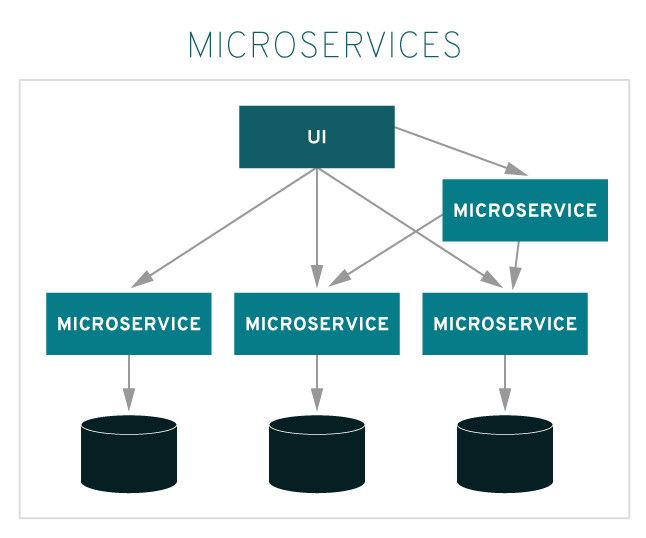
\includegraphics[width=0.55\textwidth]{monolithic-vs-microservices_altered.png}
            \caption{Structure of Microservices - [Altered], \\\textit{Source:~\cite{redhat_micro}}}\label{fig::micro}
        \end{figure}

        \subsubsection{Virtualization and Containerization}\label{sssec::virtual}
        Virtualization is an abstraction layer. The physical hardware (called host) runs a hypervisor that allows the execution of (multiple) virtual machines (called guests) which act like a regular computer~\cite{vmbasics}. This approach allows the usage of heterogeneous hardware without an impact on the guest operating systems thanks to the abstraction provided by the hypervisor. Without the need for specialized hardware and the dynamic allocation of resources, efficiency is also increased~\cite{redhat_venv}. Additionally, virtual systems can be managed more easily because fundamentally they are just one big file on the host's storage device. They can be created on command, cloned and deleted without the configuration steps of a physical system. In the enterprise industry it is common to use this flexibility to start additional \ac{VM}s on high load. According to a study by the \ac{IDC} more than 80\% of data center workloads are virtualized~\cite{virtualaddoption}. Virtualization comes with the benefit of security. The majority of hypervisors strictly separate the host and the guest system. The guest system is not allowed to use the hosts resources and access its files unless it is explicitly configured to do so. Compromising a \ac{VM} does not affect the host or any other \ac{VM}s~\cite{vmbasics},~\cite{redhat_venv}.\newline
        Full guest virtualization emulates a complete \ac{OS}, including the kernel, system libraries and even the majority of hardware devices. This abstraction comes with a performance penalty called overhead~\cite{vmbasics}. A supposedly more lightweight approach of virtualization is called containerization. Studies by Ericsson Research, Nomadic Lab~\cite{ieee_perfomance} and the Zhengzhou University~\cite{zhengzhou_university} conclude in fact that container based virtualization solutions provide better performance, especially in disk \acs{I/O} and network \acs{I/O} bound scenarios. Containerization focuses on the isolation of one application process in a virtual runtime using control groups and namespace technologies~\cite{cgroups}. Unlike \ac{VM}s, system and kernel functions are not virtualized and are passed through to the host machine. The result is a reduction of overhead and the ability to run additional application instances compared to \ac{VM}s with the same amount of compute resources. Figure~\ref{fig::vm_docker} visualizes these differences between these approaches. The left side shows a traditional \ac{VM} based approach, on top of the host \ac{OS} runs a hypervisor which provides three full guest \acl{OS}s each with one application. Each gust is fully isolated and with its own kernel, \ac{OS} and runtime libraries. The container based solution only needs the host \ac{OS} and provides multiple application instances with shared libraries and runtimes in separated, isolated namespaces.\newline
        Apart from the performance benefits, the presumably main advantage of containers is their scalability, due to faster creation and startup times~\cite{cintainer_scale}. Which makes them an adequate fit for microservices. The most popular container based virtualization solutions are Docker, Podman and LXC. A more detailed explanation of Docker can be found in Section~\ref{sssec::docker}.

        \begin{figure}
            \centering
            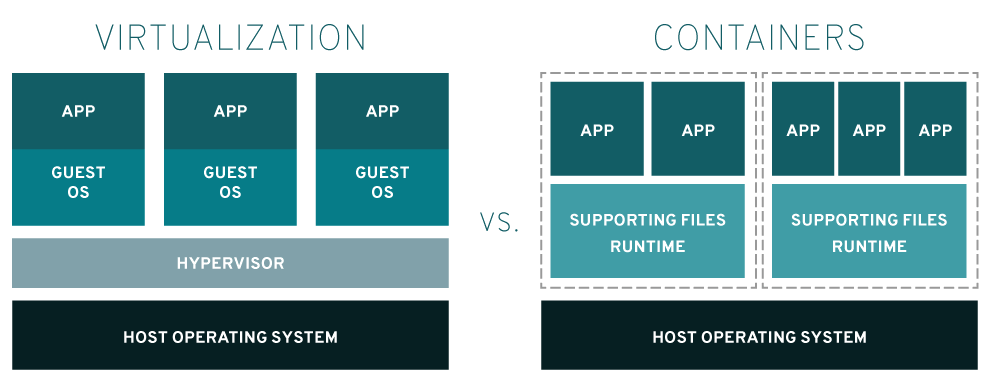
\includegraphics[width=0.9\textwidth]{docker-vm-redhat.png}
            \caption{\ac{VM}s compared to Containers, \\\textit{Source:~\cite{redhat_pic}}}\label{fig::vm_docker}
        \end{figure}

        \subsubsection{Usage of Containerization in Microservices}
        As described above, microservices are small, bounded applications that communicate with each other. To follow the principles for loose coupling between applications the communication should be performed over a programming language independent protocol. Typical \acs{IP} based protocols used are \wordhighlight{\ac{REST}}, \wordhighlight{WebSockets} or \wordhighlight{GraphQL}~\cite{micro}. These loose coupled applications have the advantage that they can be development simultaneously from different teams as well as upgraded and replaced independently. As a result, applications can be developed much faster and more flexibly, following the principles of agile development~\cite{micro},~\cite{redhat_micro}.\newline
        The usage of containers brings this speed and flexibility even further. Containers provide a consistent, isolated yet flexible runtime for applications \cite{micro_container}. Applications are packaged within known good runtimes. This reduces the setup time of the deployment and eliminate host specific errors. New application instances can be started without additional configuration. As a result of the successful concepts, tools like \wordhighlight{Docker Swarm} and \wordhighlight{Kubernetes} have been developed that can scale distributed applications in a managed dynamic, even automatic way.\newline
        \noindent Packaging and eventually even deploy the application introduces additional work for developers that was previously the task of the operations team. As already stated above, the developer and operations team are not separated in a DevOps culture. The new focus places value on team communication, flexibility and autonomy provided by the automation and support of as many steps as possible between the development and operation workflow~\cite{effective_devops}. Eliminating manual tasks allows developers to focus on the actual application development. One of the main concepts in this process is the usage of \ac{CI} and \ac{CD} workflows.

    \subsection{Tools for Archiving a DevOps Environment}\label{ssec::getting_devops}
    % TODO Adapt to new content form part 4
    \acl{CI} and \acl{CD} are two working concepts that are particularly well known in \ac{MSA}. Since every service provides only one part of the overall application functionality, it is uncertain what effects a change in one service has to other services and the whole application. Accordingly, testing must take place between applications, especially if they are developed by different teams.

        \subsubsection{Version Control}
        A \acl{VCS} (\ac{VCS}) is an essential tool in the software development industry to keep track of which change was made when and by whom. Contact persons for specific code sections are thus directly known and the responsibilities clearly defined. \wordhighlight{Git} became the defacto standard over the last 10 years and is used in the following sample project just like by over 93\% of all developers according to the StackOverflow Developer Survey 2021~\cite{stackoverflow2018}. Git allows collaborative, distributed work in own branches without affecting others. Changes can easily be merged back into the main branch after an optional review approved the changes. It is than made available for all developers. In the Symbic project, these functionalities are provided by a self-hosted instance of \wordhighlight{GitLab}. It is used to coordinate teamwork via issues and task-boards, document the project and serves as a central code repository. Its adaptability, extensive integration options and built-in \acs{CI} tools provide all the necessary software lifecycle programs from a single service bundle. Alternatives are \wordhighlight{GitHub} and \wordhighlight{Bitbucket}, both of which offer code hosting, issue management, and \ac{CI}/\ac{CD}.

        \subsubsection{Continuous Integration}
        Continuous Integration is a practice where new code is regularly integrated into the main code branch and into the overall service. Instead of having isolated functional branches that are worked on independently for months, changes flow back regularly into the main code branch to ensure it is free from conflicts and errors. Especially in interconnected services, it is indispensable to ensure that a change in one application do not have an unintended effect on other applications. \ac{CI} systems can perform automatic tasks, called jobs, on the code when it is checked into the \ac{VCS} repository. These tasks can ensure a specific code-style, run Unit or \acs{API}-tests and can also run integration tests against other services. If a task fails, the corresponding developer is notified and the changes are not incorporated into the main development branch. In case of an error it becomes easier to identify its source, due to these small and continuous integrations. Accordingly, errors and their causes can be identified more quickly and resolved without delay \cite{azuredevops}.\newline
        Popular services that provide continues integration functionality are, \wordhighlight{Travis}, \wordhighlight{CircleCI}, \wordhighlight{GitHub Actions} and the previously mentioned GitLab \ac{CI}. These services differ in their function range, type of job configuration, the level of control, whether they can be self-hosted and in their pricing models respectively the number of free jobs.

        \subsubsection{Continuous Deployment}
        Continuous Deployment on the other hand is a practice to bring these regular updates quickly and automatically into production making them available for customers. It typically involves two steps, Continuous Delivery and Continuous Deployment. The continuous creation of software bundles, called artifacts, falls under Continuous Delivery. The transfer of these artifacts and making them usable is described as Continuous Deployment. To ensure product quality, it is best to have multiple deployment environments, as described in Section \ref{ssec::devops_princibles}. Each new version is automatically deployed to a test or development environment where it undergoes automatic or manual testing. Common test types are security scans, load- usability- and acceptance tests. If all tests are successful, the version is promoted to the next deployment environment. In case of an error, the version is discontinued, and the developers are notified about it. Only if all previous environments have not revealed any errors, the version will be transferred to production as a new release. \ac{CD} is an extension of the \ac{CI} principle and performs the next logical step in the software development workflow, accordingly \ac{CI}/\ac{CD} are often used together \cite{azuredevops}. Well known \ac{CD} solution are \wordhighlight{Jenikns}, \wordhighlight{Azure Pipelines}, \wordhighlight{\ac{AWS} CodeDeploy} and \wordhighlight{Argo \ac{CD}}.

        \subsubsection{Building a streamlined workflow}
        By combining the previous principles, powerful workflows can be created that accelerate software development through automation and ensures consistent quality. Figure~\ref{fig::cd} visualizes a complete exemplary \ac{CI}/\ac{CD} pipeline. It is typically built from multiple stages, where each stage bundles one or more related tasks. A stage gets triggered by an event like code check-in or a previously successful stage. Common tasks are code style tests along unit tests, automatic compilation or packaging and the deployment to a test system.\newline
        Both \ac{CI} and \ac{CD} are practices to automate tasks that have previously been performed manually. Integration testing and packaging both have been moved to a dedicated, autonomous system, giving developers and operators more time for other activities. Deploying and using such a system are typical tasks in a DevOps practicing team. The focus here is on collaboration between the development and operations teams. Depending on the current task, new services must be added to the pipeline or existing services must be adapted to the current development status. Providing this workflow allows a team to react quickly and flexibly to changes and thus to comply with the agile principles. Through close collaboration and functioning systems, the main goal is to add value to the product and customer experience.\newline
        The GitLab instance, utilized in the following project, is used to automatically test, build and deploy the code to a testing environment. Docker images are used to bundle the individual applications, which are explained in the next section. Thus, the built-in private image registry of GitLap also allows the creation of always up-to-date Docker images and makes them accessible to all authorized entities.
        % !TeX root = ../thesis_main.tex
\begin{figure}[]
    \centering
    \tikzstyle{block} = [rectangle, draw, fill=green!80!blue!70,
    text width=5em, text centered, rounded corners, minimum height=4em]
    \tikzstyle{line} = [draw, very thick, color=black!50, -latex']

    \begin{tikzpicture}[scale=2, node distance = 5cm, auto]
        % Place nodes
        \node [block] (init) {Code Check-in};
        \node [block, right of=init] (test) {\ac{CI} Pipeline \& Code-Test};
        \node [block, right of=test] (build) {Build \& Package Code};
        \node [block, below of=build, node distance=3.5cm] (d_test) {Deploy to Testing};
        \node [block, left of=d_test] (d_staging) {Deploy to Staging};
        \node [block, left of=d_staging] (d_live) {Deploy to Production};

        % Draw edges
        \path [line] (init) -- node {Triggers} (test);
        \path [line] (test) -- node {If successful} (build);
        \path [line] (build) -- node [left]{If successful} (d_test);
        \path [line] (d_test) -- node [above]{On approval} (d_staging);
        \path [line] (d_staging) -- node [text width=2.5cm, align=center, above]{On release approval} (d_live);
    \end{tikzpicture}
    \caption{Continuous Deployment Workflow, \\\textit{Source: Modeled after~\cite{azuredevops}}}
    \label{fig::cd}
\end{figure}



        \subsubsection{Virtualization with Docker}\label{sssec::docker}
        In order to use the virtualization concepts described in Section \ref{sssec::virtual}, they have to be implemented in software. One solution for the implementation of container-based virtualization is Docker. Docker is currently the most popular containerization platform that is supported on Linux, Windows and macOS~\cite{docker_share}. It utilizes the hosts Linux kernel and its cgroups functionality for resource isolation. On none Linux host systems Docker virtualizes the kernel via a hypervisor. Docker was chosen for its wide usage, extensive documentation and its platform independency, which enables usage in local and productive operation.\newline
        Docker allows the isolated execution of applications within a container in a well-defined state without affecting the host. The initial state of a container is defined in a disk-image that bundles all the software, libraries and configuration files needed. Images are build based on a \wordhighlight{Dockerfile} that contains sequential, imperative instructions on how the container \ac{OS} should be configured. An exemplary Dockerfile can be found in the appendix in Listing \ref{code::docker}. Common steps are the \code{COPY} command to add files from the host to the container and the \code{RUN} command to execute shell commands within the container. Each instruction that changes files adds another layer to the overlay-filesystem that is used by Docker. Effectively making each layer a read only filesystem once it is written. At runtime a file-lookup is performed in the top filesystem layer, if the file is not found lookups in the layers below follow. This allows the reuse of layers, because changed versions of files are simply pushed into a new layer and overshadow the original files. Docker images are distributed via a Registry to other systems. The company that develops Docker also provides an official and public Docker image registry called \wordhighlight{DockerHub}. It provides official images of common applications such as \acl{DB}s and webservers as well as base images for own projects \cite{docker2020}, \cite{dockerdocs}.\newline
        When a container is started, the program specified in the image is executed, and the container runs until the started program exits. Each container is treated as an independent full-fledged computer with its own \ac{OS}. For this reason, each container has its own \acs{IP} address and is by default not reachable from the host. The user has to explicitly expose a container port to the host system in order to access the application inside the container. Each container not only has its own \acs{IP} address, but is also on its own virtual, software defined network, which is managed by Docker and even uses a Docker internal \ac{DNS} server. Accordingly, containers within a defined network can communicate with each other by their (host-) names and provide their functionality outside the network by exposing their published ports to the host \ac{OS} \cite{docker2020}.\newline
        Unlike \ac{VM}s, the container's guest \ac{OS} is not maintained, as containers are considered disposable. Instead of updating the software within the container, it is simply replaced by a newer one from an updated image. All changes and new files within the container will be lost. To avoid losing user data, private keys and the like, these can be stored on the host system for persistence and made available in the container via mounts. A mounted directory behaves like a new top layer in the overlay filesystem. Docker distinguishes between volume-mounts and bind-mounts. Volumes are managed by Docker, have a unique name, can easily be shared between containers and are transferable between hosts. With bind mounts a specified directory from the host is mounted to the container. All filesystem attributes and file properties are passed to the container, the management of these is up to the user \cite{docker2020}, \cite{dockerdocs}.\newline
        Alternatives to Docker are \wordhighlight{Podman}, \wordhighlight{Rkt} and \wordhighlight{LXC}, wich Docker was originally based on. The downside of these tools are their lower integrability and lack of multi-platform support.

    \subsection{Relevance of Modern Development Techniques}
    The above explained concepts are becoming more and more relevant with the increasing adoption of agile principles, even outside the software industry. The annual agile report showed a significant growth in agile adoption from 37\% in 2020 to 86\% in 2021. Key reason for adopting agile practices seem to be enhanced ability to manage changing priorities and increased speed of software delivery. The same reasons for adopting agile also apply for investing in a DevOps culture. Over 70\% of all respondents, in the annual survey, are executing or planning a DevOps initiative. One of the biggest challenges in implementing DevOps seems to be inconsistencies in processes and practices, this result is also reflected in the fragmented and heterogeneous processes described in the next section \cite{agilereport2021}.

\section{Analysis of the Current State of Development Environments}\label{sec::problem}
The following Section will display the current status of a typical development environment, point out its problems and provides approaches for possible solutions.

    \subsection{Current State of Development Environments}
    Software development involves a broad variety of tasks. Depending on the project, tasks can range from web development, desktop or mobile application development, embedded system development, data analysis or the pure maintenance of one of these variants. Each of these software development fields has its own workflows and requirements for the actual development setup. Even within these specialties, there are different requirements, depending on the scope, size, power and general capability demand for the project. Accordingly, development environments setups can differ greatly from one another. In order to limit the problem scope and possible solutions, this work will only refer to web services that are built on a microservice architecture. Nevertheless, parts of this work can also be adapted to other types of development.\newline
    Despite the increasing use of web-based \ac{IDE}s such as \wordhighlight{CodeSandbox}, \wordhighlight{StackBlitz}, \wordhighlight{Codespaces} and \wordhighlight{Gitpod}, native development environments are still primarily used. This is shown by the StackOverflow Survey, according to which Windows is the operating system primarily used by professional developers, followed by macOS and Linux~\cite{stackoverflow2021}. Accordingly, developers need a modern computer on which all the required applications must be installed and set up locally. Depending on the application area, this may include some applications for which license costs may have to be paid and which must be kept up to date after the initial installation. These are necessary supporting processes in software development, but they can cost a lot of time and effort and therefore money without producing any actual progress/value. This is especially true if there are many developers in a large company or frequently changing developers. Once the environment is running developers can start to code and contribute to the project. Programming is about changing things, changes can break things. The developers of GitHub created a series of scripts just to get developers to a working environment in less than a day. Because of frequent error these scripts included a global clean option (called \code{--nuke-from-orbit}) to reset the environment the initial known good state~\cite{githubblogcodespace}.\newline
    Such a local working environment gives developers lots of control over their development environments, compared to the functionally restricted web-based environments, but it requires much effort and results in a restricted, error-proneness's environment as the next section shows.

    \subsection{Common Issues in Modern Development Setups}
    The current congestion of development environments, as described above, is a collection of different programs and their configurations that each developer has to spent worktime on setting it up to a working state that suits their personal preferences. Only when this has been set up for the respective project developers can begin with their actual work. However, their work may be restricted by the chosen software architecture and interrupted if changes in the code or its runtime cause problems with the development environment. The following section describes the most common issues with local development environments.

        \subsubsection{The Initial Setup Process}\label{sss::initial}
        Newly recruited developers or those changing projects need time and support to settle into the new project. They are not familiar with the code base and instructions on how to set up the environments correctly. Of course, good code documentation helps, as long as it is available, up-to-date and detailed enough. Specific software packages such as \ac{DB}s, interpreters or compilers need to be installed and configured in the correct versions to make the local environment operational. Often debuggers are not included in the language framework and do not need to be installed and set up additionally. Depending on the project, this can be very extensive and require a lot of time and support from other team members. Setting up a platform independent NodeJS project is considerably simpler thanks to the included package manager \wordhighlight{npm} than it is with C++ or PHP projects. A survey by ActiveState showed that over 25\% of developers need five more hours to set up a development environment. Considering that over 65\% of developers do this one to four times a year, 30\% even five to twelve times a year, this adds up to a significant percentage of work hours \cite{setuppain}. An Internet search also reveals a wide range of discussions about automating this process exist. Further problems that arise from the configuration of the respective programming language are discussed in more detail in the next point. \newline
        Even though some of this initial work can be automated with scripts, these scripts must be created and maintained for each operating system used. These can be a time saver as long as they don't break due to moved download links or unavailable files.

        \subsubsection{Dependency Management \& Configuration Shift}\label{sssec::dependency}
        Once the development environment is set up it is a crucial job to maintain it in such a way that developers can do their real work and contribute value to the product. Some programming languages frameworks are able to keep dependencies consistent across multiple systems without much effort thanks to their integrated framework tools that come with them. NodeJS for example installs all the required dependencies locally in the project folder and keeps a precise record of their versions by means of a \code{package-lock} file. Other languages either come without any package manager at all or their package manager installs dependencies globally. The existence of tools like pythons \wordhighlight{venv} package for creating virtual isolated environments for project dependencies proof that dependency management is in fact a problem in local development environments~\cite{pythonvenv}. Apart from architectural designing, meetings and testing investigating bugs and maintaining the application setup are the tasks that consume the most amout of time when developers are not coding. Among the problems that occur, dependency issues are ranked as the third-largest group, just after of package building issues \cite{setuppain}.\newline
        Even the local package installation approach of NodeJS do not solve the problem of developing against multiple versions of the NodeJS framework. Testing a new major version of NodeJS can break existing project configurations. Undoing these changes can be tedious and time-consuming. Additional tools like the \wordhighlight{\ac{NVM}} have to be used in order to run multiple NodeJS versions on the same system. It becomes particularly problematic when developers are working on several projects at the same time and these have different dependency requirements. Legacy applications may require runtimes and libraries that are no longer supported on modern systems. Versions prior to PHP 7, for example, can no longer be installed (without extra effort) on current Windows or Linux distributions. These issues are assigned into the runtime dependency management category. In a microservice architecture, the service dependencies further extended this problem. \newline
        In a microservice architecture, there are several granular applications, each of which provide functionally related logic and has bounded endpoints. Each endpoint can be considered to be a public \ac{API}, even if the service is just accessible within the overarching service. Communication between these endpoints is called inter-service communication. Maintaining compatibility between applications becomes a challenge especially with many microservices or when using a service mesh \cite{micro}. If a team member changes the interface of one microservice it will affect other services and the developers responsible for these applications need to be notified and respond in order to avoid unexpected errors. Tools like \wordhighlight{Swagger} for applying the OpenAPI-Specification can help with these challenges. Nevertheless, the \ac{API} version that is used must be defined and configured accordingly in other applications. The management of inter-service communication has a direct impact on the testing possibilities, which are discussed in the next section.\newline
        In ideal environments, the local setup would always work as long as no changes are made. But there are always changes, \ac{OS} and security updates, changes to the dependencies to test a new version or the temporary change of the network port for a side by side comparison. The modification of the database schema by one developer can cause a broken environment for other developers. These slide changes over time are called configuration shift. No system is identical to another which can lead to unreproducible builds and fluky errors. For this reason, the popularity of tools such as \wordhighlight{Terraform}, \wordhighlight{Puppet} and \wordhighlight{Ansible} that implement the \ac{IaC} principle and rely on the automated creation and configuration of \ac{VM}s instead of manual creation is increasing in the operational cloud sector. Each instance of a machine is configured in an exact consistent way a human being could not do. If a \ac{VM} behaves abnormally, it is tern down and recreated. However, local environments are not considered disposable, they are personalized and therefor hard to automatically create and maintain. Some projects may require exact reproducibility, especially in a scientific context. This is difficult to achieve in indiscriminately configured and personalized environments.\newline
        The tools mentioned above help to keep the system in a consistent good state, but do not help much with the many changes within the application. Well-known software practices such as database migrations and test suites are required to minimize errors within applications, but testing is a particular challenge in a microservice architecture.

        \subsubsection{Increased Testing Effort}\label{sss::testing_problem}
        The goal of tests is to verify the behavior of the system under the given conditions. It is a crucial practice to ensure product quality and high custom value \cite{azuredevops}. Functional tests can be categorized into the four stage shown in Table~\ref{tab::tests}. According to the test pyramid, unit tests are the tests with the smallest scope, but which should be implemented most heavily. They ensure the correct behavior of a function or a class and only relay on the code to be tested itself. After the compiler or linter, they are the erliest stage to detect errors. In a \ac{TDD} environment the tests are even written before the application code itself to ensure the application meets the project requirements. The use of unit tests remains unchanged in a microservice architecture as each service can still have its own unit test cases. Due to the number of applications, though, \ac{IPC} in a microservice architecture increases significantly, making integration and higher testing scenarios more complex \cite{microtest}. \newline
        Integration tests should verify that two applications can successfully interact with each other. In order to perform these it is necessary to is to run both applications simultaneously \cite{azuredevops}. Triggering an \ac{API} event and verifying its result shows integration errors, but makes them as complex as end-to-end tests thanks to the configuration and orchestration of multiple services \cite{microtest}. While developers can use tools such as \wordhighlight{Postman} to check the results of an \ac{API} call, this does not guarantee that two applications can actually communicate successfully. Integration tests can either be done in \ac{CI} where an error can only be detected after code has already been committed, pushed and \ac{CI} tasks completed, or locally with immense effort for the entire configuration of all services. Due to the high rate of inter process communication, the use of tracing tools may be necessary to isolate an inter application error. Integrating tracing programes into \ac{CI} and accessing them locally is another significant technical task. This results either in very late error detection, which slows down development and makes it more expensive, or in an individual, local environment that is difficult to maintain and prone to errors. Both scenarios leave developers with insufficient testing capacities for efficient software development. Although contract testing for compliance with shared \ac{API} specifications can be used for integration testing, this merely postpones the problem to a later test stage \cite{microtest}.\newline
        Entire application tests, called end-to-end tests, are extensive and slow. They need to have all applications to be deployed to cover entire business logic operations \cite{microtest}. They should be used thoughtful and performed on a testing or staging environment. However, these only form a small part of the test scope and are typically performed by a separate \ac{QA} team. When an error is detected, its cause must be found, for which tracing and debugging programs are used. The absence or previous configuration of these tools complicates the work and is one of the problems already described above. The lack of tools and too complex, differentiated environments are also one of the main challenges in implementing DevOps practices \cite{devops_challenge}.

        \begin{table}[]
            \centering
            \begin{tabularx}{0.9\textwidth}{lX}
                Test-Type & Description \\ \midrule\midrule
                Unit test& Test a small part of a service, such as a class.\\
                Integration tests & Verify that a service can interact with infrastructure services \\
                Component tests & Acceptance tests for an individual service. \\
                End-to-end tests & Acceptance tests for the entire application.
            \end{tabularx}
            \caption{Different types of software tests, \\\textit{Source:~\cite{microtest}}}\label{tab::tests}
        \end{table}

        \subsubsection{Issues Caused by Heterogeneous Development Environments}\label{sss::hetero}
        According to the StackOverflow Survey 2021, Windows is the most used operating system for software development, but in the server area, Unix-based systems clearly dominate with market share of 75.3\% among webservers \cite{stackoverflow2021}, \cite{unixusage}. The current state of affairs is thus obvious: Develop on Windows operate on Linux. This fundamental difference in the base runtime environment of applications can be the cause of a variety of operating system specific errors, even if the used programming languages supports cross-platform compatibility. One major differences is the structure and functioning of the file system. Windows uses alphabetical identifiers like \code{c} and \code{d} for drive partitions. Linux, on the other hand, has a root directory (\code{/}) in which all underlying folders and partitions are placed. External partitions can be mounted at any place and with any name. A frequently used directory for external partitions is under the \code{/mnt} directory. Accordingly, the representation of file paths also differ. While user data under Windows can be accessed in \code{C:\textbackslash Users\textbackslash USERNAME} using backslashes, under Linux it is usually \code{/home/USERNAME} with a normal slash character. The inclusion of external libraries, assets and other files via paths is a common task in programming. Hardcoding these paths can lead to unexpected behavior on a different host. Although some programming languages offer constructs such as \code{File.Separator} or attempt to perform the path separator conversion automatically, errors still occur on heterogeneous systems. One of the reasons is the special meaning of the backslash, which is often used to escape reserved special characters.\newline
        Similar to the file paths, the encoding of the newline character differs. Windows uses the \code{CR} line ending format and Linux the \code{LF} format. There are applications that can read both encodings nevertheless, there are also applications that either only support CR or can only read LF encoded newline characters. Bash scripts created under Windows cannot be executed under Linux without a conversion from CR to LF. The permission system of Windows and Linux also differ. Windows uses the central user account control for managing read, modify, change owner and delete permissions. Linux, on the other hand, has a read, write and execute flag for the owner, group members and other users for every file. Windows does not support executable flag at all. Accordingly, all files created under Windows which are then copied to Linux environment cannot be executed without further steps. Another example for these problems is the handling of keys and certificates. The widely used key-based cryptosystem \ac{RSA} can be used under both Windows and Linux, but with differences. Keys created under windows are not accepted by many Linux applications because they cannot be read due to CR line endings or are rejected because \wordhighlight{nginx}, \wordhighlight{apache webserver} and \wordhighlight{sshd} require that private keys are only readable by the user and the permissions are too open by default.\newline
        These heterogeneous based problems come in addition to \acl{OS} specific programming. Low level operations such as forking a process, spawning a new one and sending (exit) signals are fundamentally system specific. Higher level programming languages abstract some of these operations, yet some functions are only available on one specific system such as Unix sockets. Dependencies using native lieberies are also \ac{OS} specific. They either have different variants for each host or they are compiled into native libraries on the traget system at install time like NodeJS does with \wordhighlight{node-gyp} or Python with \wordhighlight{wheels}. Having this deviating behavior adds extra complexity and creates new error sources.

        \subsubsection{Additional Effort for Developers and extra Cost}
        The above sections already show how heterogeneous environments, many small services and an extended testing effort cause additional work for developers. In addition, there is also the management of secrets such as \ac{API}-tokens or keys and, for new developers, the setup of \ac{VPN}s and communication tools. Even when the local environment runs there are ongoing obstacles. As said before the value of microservices is to have multiple small application that together provide a greater functionality. To start multiple microservice developers most likely need multiple terminals to execute each application. Having three or more terminal sessions can quickly become confusing. Eventually services even have a specific order for startup. This phenomenon is also referred to as terminal hell. However, the obstacles do not stop at the start of the individual applications; tracking their output is also one of the tasks. Log outputs provide insights into what the application is currently doing. This makes it possible to quickly check the expected behavior of an application. The output of many logs on different terminals, however, only contributes to a rapidity increasing confusion. Analogous to the terminals, this is called log hell \cite{micro}.\newline
        These circumstances lead to developers spending more time managing, configuring and analyzing applications rather than actively developing them. Which leads to a slower pace of development. Slower development increases cost and leads to customers having to wait longer for new features and bug fixes, which diminishes the customer experience. If a company's business model is to offer software development as a service, slower and higher development costs mean that the company cannot compete with rival companies and loses contracts.

        \subsection{Propsed Solution}
        The root cause of these problems is that local development environments fundamentally differ from production environments. Local environments are deeply individualized and personalized, while production environments are scandalized but very complex. Local environments cannot be set up automatically and thus cannot simply be torn down and replaced in the event of errors. Long troubleshooting sessions are the consequence resulting in a slow-down of the development progress.\newline
        In the server world, virtualization technology is used for uniform and well-defined environments. With tools like Terraform or Ansible, any number of server instances can be created in a short time in exactly the same configuration. A constant and isolated application runtime environment is provided by a virtualization solution such as Docker and applications are orchestrated and scaled with a Docker Swarm or Kubernetes cluster.\newline
        This thesis proposes to use exactly this virtualization approach for local development environments. Thus, the configuration effort, the lack of testing possibilities and the occurrence of local and operating system specific errors should be reduced.

\section{Solution Concept of DevContainers}\label{sec::solution_concept}
This section proposes the usage of Development Containers (DevContainers) as a solution to the problems of local development environments described in Section \ref{sec::problem}. The concept is oriented according to the \ac{PaaS} principles known in the cloud. Developers should only have to deal with the application. The runtime environment and network configuration are managed by the DevContainer. They combine the application runtime and its configuration into an isolated environment by using the lightweight virtualization approach of containers. One difference between DevContainers and the \ac{PaaS} principle is that DevContainers do not provide own hardware neither its management. \newline
The details of such a DevContainer concept are described below. This is followed by a delimitation of when its application scenarios make sense and when they do not. Finally, the advantages and limitations of this solution are outlined.

    \subsection{Description of a Conceptual Environment}
    The idea of DevContainers is to bundle the application code, its runtime and configuration into an isolated system. Only the minimal necessary scope for accessing the application are made available on the host system, everything else remains isolated. As with \ac{VM}s and containers, these can be started and stopped as required while the application and the runtime within the container has no influence on the rest of the system. When the container is started, all port, path and secret configurations are already set. No manual configuration and no further steps by the developer need to be made. Different branches and versions of the applications all have their own container which are completely independent of the local settings. Auxiliary applications and interdependent services can all be started simultaneously and in the correct order. The DevContainer environment builds upon the Linux kernel and is completely independent of the host \ac{OS} and thus much closer to the production environment, potentially decreasing system specific errors. Even if something goes wrong and the environment ends up in an undefined state, the principles from the server world can be applied. The DevContainer can simply be discarded and recreated from a well-defined template within seconds. Which even can enable environments that are 100\% reproducible.\newline
    Such a setup allows developers to choose any host \acl{OS} because all the application code is in a virtualized environment. It increases the initial setup time and prevents configuration drift because all configuration settings are following the \ac{IaC} principle and are stored as code. This way, new runtimes or dependencies can be tested without having to risk corrupting the local environment. Through automatic orchestration, integration tests become easier and can be performed earlier, shortening the time until an error is detected. Dependencies and common software like debugger are already present in the container, so they do not need to be installed separately. DevContainers promise to solve the problems described in Section \ref{sec::problem} and allow developers to focus on programming rather than configuring and maintaining their working environment.\newline
    Despite these potential advantages, DevContainers are not the miracle solution to all problems in software development. They have their limits and their area of application wich they are suitable for.

    \subsection{Pre-requirements for DevContainers}
    Before the use of DevContainers one has to verify hat these are the right approach for the encountered problems and that all necessary requirements are fulfilled.\newline
    DevContainers are based on virtualization technology, and one of their goals is to achieve the greatest possible similarity between the development and production environments. In order to take full advantage of this possibility, the production environment must already be designed for the use of virtualization with containers.  As can be seen in Section \ref{ssec::toolsused}, the majority of virtualization solutions are based on Linux, which is also the most widely used system in the server domain. Applications that require Windows can also use Windows-based containers, but these may require additional licenses and configuration, accordingly they will not be discussed further in this paper. The application to be developed must be suitable for use in a container. Containers do not offer direct support of graphical output by default. Functions are exposed to the outside world via the usage of sockets or mounted devices. Experience in the area of virtualization and a functioning \ac{CI}/\ac{CD} pipeline for the rapid delivery of new application versions is therefore also recommended.\newline
    Although DevContainers reduce the configuration effort for each developer, the architecture and settings files for the use of DevContainers must be created once and then be maintained. As Section \ref{sssec::virtual} already shows, with any kind of virtualization, regardless of whether it is VMs or containers, there is a performance overhead. If, as in a typical microservice architecture, several applications are run at the same time, this overhead adds up and places an additional load on the developer's system. Modern hardware with sufficient memory and computing capacity is therefore necessary for the use of DevContainers. The amount of additional load depends on the technology stack used.

    \subsection{Creating a DevContainer setup}\label{ssec::toolsused}
    Section \ref{ssec::getting_devops} already presented concrete programs for providing the virtualization concept and automating certain processes with \ac{CI}. These form the basis for the provision of DevContainers. This must now be made available to developers in actual concepts and, in doing so, solve further problems described in Section \ref{sec::problem} as good as possible. Developers need to be able to interact with the DevContainers and especially their applications without significantly impacting their workflow. Therefore, tools and concepts that make this possible are presented below.

        \subsubsection{Interacting with DevContainers}
        The primary way developers interact with their code and the application is through their editor. Their variability and the number of different editors is great. Well known general purposes editors are Visual Studio, XCode, Atom, Sublime, Eclipse, Emacs and VIM. There is usually a distinction between simple text editors and \acl{IDE}. While text editors are quite simple and only provide basic functionalities like syntax highlighting, \ac{IDE}s are much more comprehensive with powerful IntelliSense suggestions, built-in project management, \ac{VCS}, debugger, graphical visualization and build-tools. The choice of the editor is a personal decision for most developers, and they are customized according to their preferences. For this reason, the proposed solution does not require a specific editor for DevContainers, but gives a recommendation that will be used as a reference for the rest of the work.\newline
        \ac{VSCode} is a free platform independent editor with extensive extendibility which is used by over 70\% of all developers accordingly to StackOverflow~\cite{stackoverflow2021}. One of its key beneficial features for virtualized work environments is its Remote Development functionally. This, officially provided, extension provides the comfort of a graphical \ac{UI} while running the code, the application and auxiliary processes like a debugger on another, remote machine. As Figure \ref{fig::vscoderemote} shows, the \ac{VSCode} frontend connects to the remote machine and installs a server instance of the editor. The server side instance manages access to the file system and the execution of other processes while communicating with the local \ac{VSCode} instance for comfortable access to these functions \cite{vscodedevcontainer}. To access services running on the remote server the extension provides a functionality to make these remote processes available locally via port forwarding. This allows the usage of local testing or exploration tools on these remote services. This type of remote development works for \ac{SSH} connections, the \ac{WSL}, and on Docker containers. \ac{WSL} is a built-in Windows feature to provide a Linux environment on Windows hosts without the need of a separated \ac{VM}. The implementation of Docker for Windows is build upon this functionality. Details on the use and configuration of this function are described in detail in Section \ref{ssec::imp_process}. All these functions can be used without \ac{VSCode} by using remote filesystem mounts, (\ac{SSH}) port-forwarding or terminal based editors. Using other editors than \ac{VSCode} may additional configuration effort or require slight implementation modification compared to the setup in Section \ref{ssec::imp_approach}.

        \begin{figure}[]
            \centering
            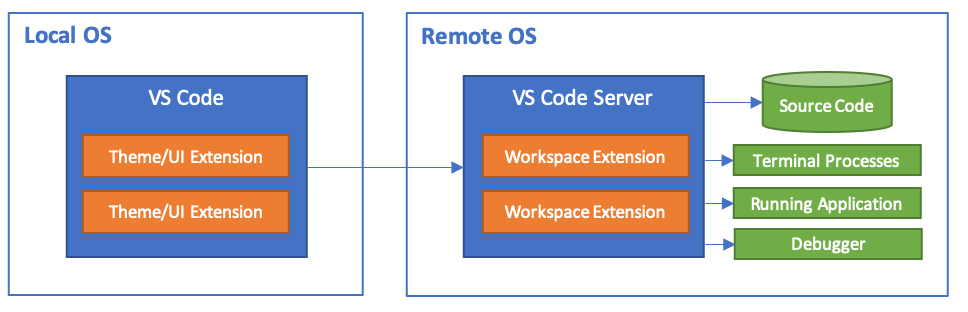
\includegraphics[width=.95\textwidth]{vscode-remote.png}
            \caption{Structure of \ac{VSCode} remote Development setup \\\textit{Source:~\cite{vscodedevcontainer}}}\label{fig::vscoderemote}
        \end{figure}

        \subsubsection{Additional Supporting Tools}
        In addition to the tools mentioned in Section \ref{ssec::getting_devops} and above, other auxiliary programes are used. To simplify certain workflows and automate recurring tasks scripts will be used. The \wordhighlight{Bash} scripting language can be used natively on Linux and macOS, the installation of Git for Windows also brings Bash support to Windows. Accordingly, one scripting language can be used to perform platform-independent operations on different repositories and simplify complex build instructions. \wordhighlight{Docker Compose} follows the same approach and facilitates the management of multiple interrelated Docker projects. It is a program for orchestrating multiple Docker containers. It ensures that interdependent services are started in the correct order and that all necessary persistent volumes are created \cite{docker2020}, \cite{dockerdocs}. Its configuration is typically specified in a \code{docker-compose.yml} file that follows the \ac{IaC} principle and is tracked in \ac{VCS}. An optional feature is to further organize the logs from all docker containers. Although Docker Compose offers color-coded log outputs per container, even these can become overwhelming if there are many containers. Since the Docker stack is used anyway, enterprise log aggregators and analysis tools like \wordhighlight{Grafana} or \wordhighlight{Elastic Search} can be used to get a persistent and searchable log dashboard. In this concept, a Grafana container is used that gets its logs from the \wordhighlight{Loki} log-shipper via a Docker plugin.

    \subsection{Strengths, Weaknesses and Limits}\label{ssec::limits}
    The software and methods described in Section \ref{ssec::toolsused} are already standard practice for many teams which are following the DevOps culture. Accordingly, the entry barrier is small in compared to new and unknown tools. DevContainer allow for a homogenization of development and production environment. The application runtime is identical, accordingly \ac{OS} or runtime specific errors are prevented. Developers can use a ready to go development project setups without having to install and configure the application runtime themselves. Dependencies, keys, supporting tools like debuggers and configurations can already be shipped within the container to enable a quick initial setup. Instead of examining the environment for a long time in the event of an error it can quickly been torn down and recreated into a known good state. These are the key features that DevContainer promise to provide, in addition to solutions to the problems described in Section \ref{sec::problem}. They extend the existing toolset of agile and DevOps teams with another tool that allows developers to be more flexible and focus more on coding.\newline
    It should be noted that DevContainers are not a perfect solution to all problems in the software development stack. Like any other tool they come with their own set of quirks. Expertise for the use of Docker containers must be available, and the production architectural must be transformable to a local DevContainer-based configuration. This configuration must be kept up to date and be maintained. Developers may need to adapt to minor adjustments in their workflow. The CI/CD solution used must always be available and provide up-to-date container images. Every virtualization approach creates an additional overhead that cannot be ignored, especially when using multiple containers on Windows based systems. Details of the exact effects are given in Section \ref{sec::eval}.\newline
    As mentioned before, there are also projects for which the use of DevContainers is simply not suitable. Heavy monolithic applications are not in the sense of containers and therefore not suitable for DevContainers. Graphical applications can run in containers but require a graphical X-Server on the host and the resulting experience is not comparable to a native \ac{UX}. Similar limitations apply to applications that require a Windows stack. This can be implemented, but is no longer platform-independent, requires additional licenses and further adaptations. For embedded projects that require specific hardware, a virtualization approach is just not feasible and accordingly these are also not suitable for DevContainers.\newline
    To demonstrate a suitable use of DevContainers, the next section describes how to migrate from a traditional development environment to a DevContainer-based solution based on a real project.

\section{Exemplary Prototype Implementation}\label{sec::solution_code}
This section descripts the implementation of the DevContainer concept on a real project that is currently developed by the Symbic GmbH. At the beginning, the initial state of the project is described and what goal is to be achieved. Then the concept from Section \ref{sec::solution_concept} is applied and an architecture for the DevContainer setup is designed. The following section describes the implementation process and places special emphasis on possible errors that can occur and what ticks there are to minimize them. Finally, the end state is compared with the previously set goal.

    \subsection{Projekt Information and about its Initial \& Target State}
    % Name for the project
    The project presented here is currently developed and maintained by Symbic GmbH. It is a system for deploying and managing \ac{IoT} devices from the agricultural sector and is based on a microservice architecture. Various \ac{API}s provide different functionalities, which are made available by multiple microservices. For its operation, various auxiliary services are required, including SSH Server and MQTT Broker. For the sake of clarity, only a subsection of the system is presented in this paper. This makes a further realistic implementation possible without going into an excessive description of the system which would take place to the detriment of the DevContainer concept. A detailed description of the project is given in the following section. \newline
    The goal is to test the concept described in Section \ref{sec::solution_concept} for applicability in a real project. The challenges encountered are described and possible solutions to them are noted. How the end state is and how it differs from the start state is explained in Section \ref{sssec::goal}.

        \subsubsection{About the Project}
        % !TeX root = ../thesis_main.tex
\begin{figure}[]
    \centering
    \tikzstyle{block} = [rectangle, draw, fill=green!80!blue!70,
    text width=5em, text centered, rounded corners, minimum height=4em]
    \tikzstyle{line} = [draw, very thick, color=black!50, -latex']

    \begin{tikzpicture}[
        align=center,
        scale=0.2,
        node distance=3.5cm,
        auto]

        % Frontend
        \node [] (user) {
\includegraphics[width=.08\textwidth]{fig/user.png}\\User};
        \node [block, left of=user, xshift=-15mm] (webapp) {
\includegraphics[width=.5\textwidth]{fig/vue.png}\\WebApp};

        % Microservice Cluster
        \node [block, below of=webapp, xshift=-20mm, yshift=-5mm] (authbackend) {
\includegraphics[width=.4\textwidth]{fig/php.png}\\Auth-Backend};
        \node [block, below of=webapp, xshift=20mm, yshift=-5mm] (deviceapi) {
\includegraphics[width=.7\textwidth]{fig/node1.png}\\System-API};
        \node[draw,dashed,fit=(authbackend) (deviceapi), label={[above]MS\\Cluster}] (microcluster) {};

        % MQTT Service
        \node [block, right of=deviceapi, xshift=2mm] (mqttcon) {
\includegraphics[width=.7\textwidth]{fig/node1.png}\\MQTT Connector};
        \node [block, right of=mqttcon, xshift=7mm] (mqttbroker) {
\includegraphics[width=.3\textwidth]{fig/mqtt-logo-small.png}\\MQTT Broker};
        \node[draw,dashed,fit=(mqttbroker) (mqttcon), label={[above]MQTT\\Service}] (mqttservice){};

        % DB Stuff
        \node[database,label=below:SQL\\User \acs{DB},database radius=.8cm,database segment height=0.42cm, below of=authbackend] (userdb) {};
        \node[database,label=below:Logs\\Mongo\acs{DB} ,database radius=.8cm,database segment height=0.42cm, below of=webapp, yshift=-38mm] (logdb) {};
        \node[database,label=below:SQL\\Device \acs{DB},database radius=.8cm,database segment height=0.42cm, below of=deviceapi] (devicedb) {};

        % Device
        \node [below of=mqttbroker] (device) {
\includegraphics[width=.1\textwidth]{fig/device.png}\\Devices};

        % Edges & Paths
        \path [line] (user) -- node [text width=2.5cm, align=center, above]{Interacts\\with} (webapp);
        % To APIs
        \path [line] (webapp) -- node [text width=3.5cm, align=center, left, yshift=3mm, xshift=4mm]{Validates Authentication} (authbackend);
        \path [line] (webapp) -- node [text width=4cm, align=center, right, yshift=3mm]{Provides Device Data \& Functionality } (deviceapi);
        % To DB
        \path [line] (authbackend) -- node [text width=2cm, align=center, left, yshift=-2mm]{Connects to} (userdb);
        \path [line] (authbackend) -- node [text width=1cm, above,xshift=10mm, yshift=-5.5mm]{Event Logs} (logdb);
        \path [line] (deviceapi) -- node [text width=1cm, above, xshift=-3.5mm, yshift=-1mm]{} (logdb);
        \path [line] (deviceapi) -- node [text width=2cm, align=center, right, yshift=-2mm]{Connects to} (devicedb);
        % MQTT Device
        \path [line ] (microcluster) -- node [align=center, above] {Uses} (mqttservice);
        \path [line ] (mqttcon) -- node [text width=2cm, align=center, above] {\acs{REST} API for} (mqttbroker);
        \path [line,transform canvas={xshift=2mm}] (device) -- node [text width=2.5cm, align=center, right]{} (mqttbroker);
        \path [line, transform canvas={xshift=-2mm}] (mqttbroker) -- node [text width=3cm, align=center, left, yshift=-3mm]{Subscribe\\\& Publish\\Messages} (device);

    \end{tikzpicture}
    \caption{IoT Web Service Architecture}\label{fig::arch}
\end{figure}


        As described above, the project used here is built on a microservice architecture. The advantage of this architecture is that it allows different technologies to be used for individual applications. Communication then takes place via a platform-independent protocol. If the load on a part of the application becomes critical, new instances of this application can simply be created and added to the service.\newline
        To allow an easier understanding of the service, Figure~\ref{fig::arch} shows its structure. Users of this platform only directly interact via the web interface with the subsection of the system that is dealt with in this thesis.
        The web interface is created with the \ac{JS} framework Vue.js which generates a static bundle of HTML and \ac{JS} files which are served by a simple webserver. To access the system, users must authenticate themselves in the WebApp. This is done via a backend written in PHP. In addition to authentication, this backend also performs other tasks which will be neglected in this work. Provided the user is authenticated, the WebApp can display internal information and functions of all deployed \ac{IoT} devices. These dynamic information are provided by the \wordhighlight{NodeJS} based SystemAPI. All \ac{API} endpoints are implemented under the compliance with the \ac{OAS}. The \ac{OAS} allows for easy discoverability and understanding of the \ac{API} for humans and computers. It also provides versioning support of \ac{API}s to avoid unexpected errors in other applications. \newline
        Both the authentication app and the system \ac{API} have their own SQL databases that persistently provide the relevant information. However, both applications write certain changes made by the user to a shared event database. MongoDB is used providing a NoSQL database with a flexible schema. To send specific instructions to or receive information from a \ac{IoT} device, the system \ac{API} communicates with an MQTT broker via the NodeJS based MQTT Connector. The MQTT Connector provides a unified \ac{REST} \ac{API} for publishing and subscribing messages over the MQTT protocol. On a larger scale, the MQTT Connector is used by several applications and is therefore a standalone application, but since only a part of this project is considered here, the System API is the only one that uses the MQTT Connector. The MQTT Broker is a public endpoint that offers various topics wich the devices subscribe or publish to. Via this system, the user can trigger a command in the web app, which is then processed and logged by the system \ac{API}. It is than made available via the MQTT Connector on the MQTT Broker. IoT devices which have subscribed to the corresponding topic receive this command and execute it. The result is published to another topic and can be accessed in the same way via the WebApp. Since the IoT devices are connected to the Internet via SIM cards, and are therefore in an own restricted mobile carrier network, they are not directly accessible from the Internet. Through the described system, the IoT devices can execute commands from the outside without being accessible via the Internet.

        \subsubsection{Initial State of the Projects Development Environment}
        New developers joining the project have to clone all four Reposition, install NodeJS and a specific version of the \ac{XAMPP} stack and customize its configuration. The details of this must be taken from the documentation, if available or are provided by a collaborator. To test the whole unified system developers also need to install a MQTT broker and the MongoDB database. Both applications need an initial administrator user which needs to be created, and the corresponding credentials need to be accessible by each \ac{API}. Then a database and its schema must be created. Eventually network ports have to be adjusted and secrets for signing tokens have to be created.
        The access data for the databases must be created in each case, the ports of the individual applications must be coordinated and possibly secrets must be entered. These steps are necessary to just get the project running properly, the setup of developer tools like debugger has not been considered yet. Even in a small project this can take some time especially if one is not yet familiar with the project.\newline
        Even experienced project members experience challenges when working on such a project. Before the APIs can be launched, it must be ensured that the databases and other auxiliary tools are already running. To start all four applications (WebApp, Auth-backend, System-API, MQTT-Connector) a developer needs four terminal sessions or a terminal multiplexer to operate all applications. The program outputs (logs) are distributed over all four sessions and cannot be directly linked to each other, neither are they filterable nor searchable. When everything is running developers can now contribute value to the project. These restrictions would be acceptable as long as the work is not interrupted by a possible error case. A merge containing dependency or database schema updates by a team member can cause the environment of others to break. Error searching in very different setups is the result. The lack of consistent, reproducible setups is the cause for lasting troubleshooting sessions and the well-known iconic saying \textit{"But it works on my machine"}. This mirrors the problems of heterogeneous systems from Section \ref{sec::problem}. It does not matter whether the individual development environments differ or the development environment to the production environment. The fact that there are always differences is the cause of this kind of problems. \newline
        These are the problems developers may experience through just one project. When working on multiple projects, the problem scope increases accordingly. Different databases, runtimes and dependencies further contribute to a greater potential for issues. The lack of project isolation may result in unintended side effects between projects that slow down the development process. To prevent unnecessary slowdowns, the initial setup of an environment and its operation must be as homogeneous as possible.
        % % !TeX root = ../thesis_main.tex
% \subsection{Figure Alternatives}
\begin{figure}[!h]
    \centering
    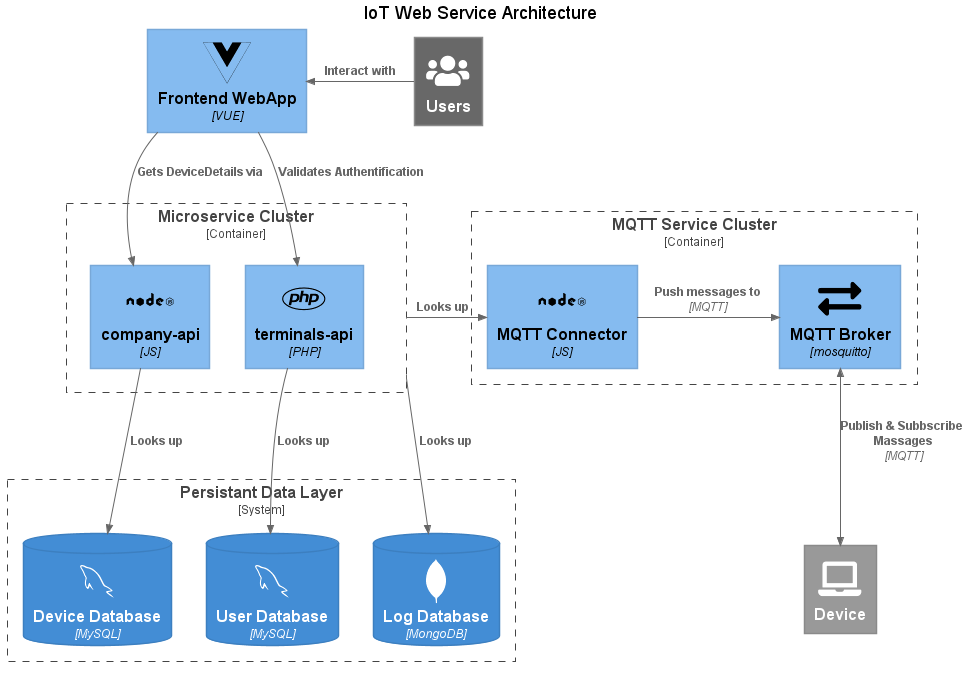
\includegraphics[width=.95\textwidth]{CCI-System-clean.png}
    \caption{IoT Web Service Architecture - [Alternative]}\label{fig::arch}
\end{figure} % Alternative
        \subsubsection{Goal for the Target State}\label{sssec::goal}

    \subsection{Implementation Approach}\label{ssec::imp_approach}
    \begin{figure}[]
        \centering
        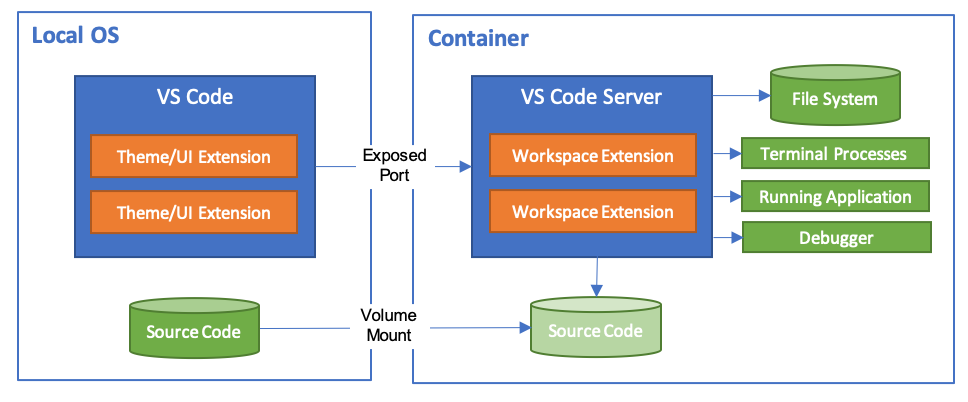
\includegraphics[width=.9\textwidth]{architecture-containers.png}
        \caption{Architecture of \ac{VSCode} container Development setup \\\textit{Source:~\cite{vscodedevcontainer}}}\label{fig::vscodecontainer}
    \end{figure}

    \subsection{The Implementation Process}\label{ssec::imp_process}
    \subsection{Encountered Challenges and Limits}
    \subsection{Final State}\label{sec::final}
%     \begin{lstlisting}[language=bash, frame=single, backgroundcolor=\color{codebg}]
% Here is the codes format i want to show in latex
%     \end{lstlisting}


\section{Performance Evaluation and Analysis}\label{sec::eval}
    \subsection{Metrics and how to Evaluate}
    \subsection{Evaluation and Results}
    % Adding a local environment increases the overall amount of configuration effort, requiring a reliable, efficient way to manage it.
    \subsection{Discussion of Evaluation}

\section{Future Potential and Outlook}\label{sec::outlook}
\section{Conclusion}\label{sec::conclusion}


% STATS
% 10000 Words
% 56.800/66.800 Characters

\newpage
% Anhang
\singlespacing{}
\lhead{Appendix}
\renewcommand{\thesubsection}{\Alph{subsection}}
\pagenumbering{Roman}
\setcounter{page}{\value{lastroman}}
\section*{Appendix}
\addcontentsline{toc}{section}{Appendix}

% Abbreviations
% !TeX root = ../main.tex
\newcommand{\abbr}{Abbreviations}
\subsection{Abbreviations}
%\addcontentsline{toc}{subsection}{Abbreviations}

\begin{acronym}[1234567890]		%[längste Abkürzung]
\setlength{\itemsep}{-\parsep}	% sorgt dafür, dass das Verzeichnis kompakt dargestellt wird.

\acro{BLEST}[BLEST]{BLock ESTimation}
\acro{CWND}[CWND]{Congestion Window}
\acro{DAPS}[DAPS]{Delay-Aware Packet Scheduler}
\acro{ECF}[ECF]{Earliest Completion First}
\acro{HTTP}[HTTP]{Hypertext Transfer Protocol}
\acro{ISP}[ISP]{Internet Service Provider}
\acro{IETF}[IETF]{Internet Engineering Task Force}
\acro{LRF}[LRF]{Lowest-RTT-First}
\acro{MSS}[MSS]{Maximum Segment Size}
\acro{MPTCP}[MPTCP]{Multipath TCP}
\acro{MPTCPSW}[MPTCP\textsubscript{SW}]{MPTCP's send window}
\acro{OTIAS}[OTIAS]{Out-of-Order Transmission for In-Order Arrival Scheduler}
\acro{RR}[RR]{Round Robin}
\acro{RTT}[RTT]{Round Trip Time}
\acro{SCTP}[SCTP]{Stream Control Transmission Protocol}
\acro{sRTT}[sRTT]{Smoothed RTT}
\acro{STTF}[STTF]{Shortest Transfer Time First}
\acro{TCP}[TCP]{Transmission Control Protocol}
\acro{VoIP}[VoIP]{Voice over IP}
\end{acronym}
\newpage

%Code
% !TeX root = ../thesis_main.tex

\subsection{Code Listings}
% \addcontentsline{toc}{subsection}{Code for you}
\begin{lstlisting}[language=docker, frame=single, caption={Exemplary NodeJS Dockerfile},label=code::docker]
# The base image to start from
FROM ubuntu:18

# Install nodeJS
RUN apt-get update && apt-get install -y nodejs npm

# Copy content of the HOSTS "backend" folder
# to the "app" folder in the container
WORKDIR /app
COPY backend /app

# Install all node-modules
RUN npm install

# Spcify the command that is run
# when the container is started
ENTRYPOINT [ "npm", "start" ]

\end{lstlisting}


\begin{lstlisting}[language=docker-compose-2,caption={Example docker-compose.yml},breaklines=true,label={code::compose}]
version: "2"
  services:
    web:
       build: .
       ports:
          - "5000:5000"
       volumes:
          - .:/code
          - logvolume:/var/log

    redis:
       image: redis

  volumes:
    logvolume:
\end{lstlisting}

% !TeX root = ../thesis_main.tex
\begin{figure}[]
  \begin{forest}
      for tree={
        font=\ttfamily,
        grow'=0,
        child anchor=west,
        parent anchor=south,
        anchor=west,
        calign=first,
        edge path={
          \noexpand\path [draw, \forestoption{edge}]
          (!u.south west) + (7.5pt,0) |- node[fill, inner sep=1pt] {} (.child anchor)\forestoption{edge label};
        },
        before typesetting nodes={
          if n=1
            {insert before={[,phantom ]}}
            {}
        },
        s sep=1.5pt,
        fit=band,
        before computing xy={l=15pt},
      }
    [ProjectRoot
      [manage-reop
        [configs]
        [scrips]
        [docker-compose.yml]
      ],
      [auth-repo
        [src]
        [vendor]
        [Dockerfile]
        [composer.json]
      ],
      [device-repo
        [src]
        [node\_modules]
        [Dockerfile]
        [package.json]
      ],
      [mqtt-con-repo
        [src]
        [node\_modules]
        [Dockerfile]\
        [package.json]
      ],
      [webapp-repo
        [src]
        [node\_modules]
        [Dockerfile]
        [package.json]
      ],
      [docker-compose.yml \textit{(symlink)}]
    ]
  \end{forest}

  \caption{Directory Structure of the Project}
  \label{fig::dirstructure}
\end{figure}
\newpage
\listoffigures
\listoftables
\lstlistoflistings{}
\newpage

%Bibliographie
\addcontentsline{toc}{section}{References}
% \bibliographystyle{alpha}
\bibliographystyle{IEEEtranSA}
\bibliography{bib/sources}

% Authorship
% !TeX root = ../main.tex
\section*{Declaration of Authorship}

\vspace{5cm}

~\\
I hereby declare that the paper submitted is my own unaided work. I assure that I wrote this paper without using any other means and sources than those specified. As well as the sources used literally or analogously taken from the sources identified as such.

\vspace{3cm}
\begin{flushright}

\rule{8cm}{0.2mm} \\
Signature (\myName)
\end{flushright}

\vspace{2cm}
\place, the \submission{}

\end{document}
% END DOC/EOF
